% First complete TeX-first Paper 1 draft; aggregate evidence only.
% Build from this directory: pdflatex Paper1_SNAM; bibtex Paper1_SNAM;
% then run pdflatex Paper1_SNAM three more times to resolve all references.
\documentclass[10pt]{article}
\usepackage[T1]{fontenc}
\usepackage[utf8]{inputenc}
\usepackage{lmodern}
\usepackage{amsmath,amssymb,booktabs,graphicx,geometry,longtable,array}
\usepackage[round,authoryear]{natbib}
\usepackage{url}
\usepackage[hidelinks]{hyperref}
\geometry{margin=1in}
\graphicspath{{figures/}}
\setcounter{secnumdepth}{3}
\setcounter{tocdepth}{2}
\setlength{\emergencystretch}{2em}
\newcolumntype{P}[1]{>{\raggedright\arraybackslash}p{#1}}
\newcommand{\ind}{\mathbf{1}}
\newcommand{\logitinv}{\operatorname{logit}^{-1}}
\newcommand{\Mfour}{\mathrm{M4c}}
\newcommand{\Mzero}{\mathrm{M0}}
\title{Exponential Random Graph Models as a Benchmark for Directed Link and Hyperlink Prediction under Missingness}
\author{[AUTHOR COMPLETION REQUIRED: names and affiliations]}
\date{}
\begin{document}
\maketitle
\begin{abstract}
Directed interaction records, their dyadic projections, and algebraically derived groups are non-equivalent prediction targets. We develop a missingness-centred benchmark that separates directed dyadic footprints, capped formal concepts, and native ordered tail/head event types. The primary data are a strict 1998--2002 Enron internal-custodian core and a 30-day analyst-defined MathOverflow answerer-to-asker reconstruction. Each fixed core is evaluated using 30 event-first masks per mechanism: uniform fixed-count MCAR and oracle activity-dependent MNAR-out stress tests. Random arity-matched panels, reversal and role-exchange panels, and fixed-participant role assignment distinguish footprint ranking from orientation recovery. On balanced random panels, the predeclared geometric ERGM conditional-footprint score improves PR-AUC over the density reference by 0.3584 and 0.3324 in Enron, and 0.2396 and 0.2394 in MathOverflow, under MCAR and MNAR-out respectively. Whole-mask bootstrap intervals are positive in all four within-fixed-network comparisons. However, random-panel gains do not transfer uniformly to directed hard panels. Capped formal concepts have zero exact event-type matches in both cores despite footprint Jaccards of 0.8567 and 0.6634. These findings support conditional footprint discrimination, not calibrated native-event probabilities or recovery of recorded groups. A two-transition chronological MPLE status check remains diagnostic only; no forecasting, neural benchmark, or MCMC-derived higher-order joint result is claimed.
\end{abstract}
\noindent\textbf{Keywords:} directed networks; hyperlink prediction; exponential random graph models; network missingness; formal concepts; native events

% MAIN PROSE START
\section{Introduction}
Missing directed interactions present a measurement problem before they present a ranking problem. An absent arc may indicate an unobserved contact, a contact outside the chosen actor boundary, or a relationship that did not occur in the retained data. A missing group record can be more ambiguous still: some of its induced arcs may remain visible through other records, while its participant set and orientation disappear. Network omission and boundary specification can alter structural summaries in ways that depend on the observation process \citep{kossinets2006}. The usual missing-data distinctions also require an explicit account of what is observed and what governs its omission \citep{rubin1976}. Here these considerations motivate controlled missingness experiments. They do not identify the actual observation mechanism of either source corpus.

Classical link prediction ranks candidate dyads using information in an observed graph, often through proximity or neighbourhood structure \citep{libenNowellKleinberg2007,luZhou2011}. Directed data require more than changing the notation on an undirected score. A source's successors, a target's predecessors, shared recipients, and shared initiators represent different relations. Reciprocity can be informative even when common-neighbour closure is weak, and activity in one role need not imply activity in the other. These distinctions affect both predictors and evaluation. A randomly sampled absent ordered pair can be easy to separate from a held-out interaction while an alternative involving the same actors in exchanged roles is difficult. Good random-panel ranking therefore does not settle whether a method recovers direction.

The problem becomes sharper when a record involves several actors. An email records one sender and a recipient head; grouping distinct answers to a question produces an answerer tail and an asker head under a declared reconstruction rule. An aggregate directed graph retains the union of the induced pairwise relations, but not the partition of those relations into records. The same graph can result from a single multi-recipient event or from several separate contacts. Repeated records and their times are also lost in a binary projection. A directed hyperlink benchmark must consequently state whether its label is a missing dyad, a derived group in the aggregate relation, or an ordered group type available from the underlying records.

This paper develops a target ladder with those three levels. The first is the directed dyadic footprint: the arcs induced by a candidate ordered tail/head pair. The second is a cap-first formal concept, obtained by applying a Galois connection to a directed binary incidence context. The third is a native ordered tail/head event type, defined from the data's record representation before dyadic aggregation. ``Native'' describes the benchmark's event layer, not a universal assertion that every dataset directly observes collective action. Enron supplies retained sender--recipient records. MathOverflow supplies an explicitly reconstructed answer-window object. Both permit an event-first masking design, but their substantive interpretations remain different.

Formal concepts are useful here because they supply a reproducible group target without pretending to recover the record stream. Formal concept analysis identifies closed extent--intent pairs in a binary context \citep{ganterWille1999}. In the directed context used below, these pairs are maximal all-ones tail/head rectangles. Their maximality can combine ties contributed by many events, or expand an event footprint by incorporating additional actors. That is a meaningful structural representation, not evidence of a recorded group. Our fidelity audit tests exact ordered-set equality as well as footprint overlap, so that a favourable dyadic agreement cannot silently become an event-recovery claim.

Exponential random graph models (ERGMs) provide a structured comparator to local directed scores. They express graph probabilities through sufficient statistics and yield a local conditional logit in terms of dyad change statistics \citep{wassermanPattison1996,krivitskyEtAl2011}. Mutuality, degree heterogeneity, directed closure, and cyclic structure can then enter a common scoring framework. However, the model's mathematical joint form and the estimator used in a benchmark are separate matters. Maximum pseudolikelihood estimation (MPLE) fits a product of single-dyad conditional terms; with dependent ties, that objective differs from the full likelihood \citep{vanDuijnEtAl2009}. We use MPLE-based conditional scores, not an unqualified claim that fitted multi-dyad scores are joint event probabilities.

The primary experiment withholds complete ordered event types before rebuilding the graph. This prevents an identical repeated type from appearing on both sides of a split. It also exposes a feature obscured by arc deletion: a held-out type's entire footprint can survive through other observed types. We compare local directed heuristics and split-specific ERGM footprint summaries on the same frozen masks. Uniform fixed-count masks and a predeclared oracle activity-biased mask supply two assumption-indexed stress tests. The latter deliberately uses full-data tail activity in selecting omissions, but scoring and fitting use only the retained graph. Thus oracle information defines the experiment; it is not a predictor input.

The evaluations are designed to separate claims rather than produce an overall winner. Random arity-matched panels assess native-type labels against sampled non-types in a defined local candidate universe. Reversal and role-exchange panels ask whether discrimination persists when orientation or role allocation is the principal difference. Fixed-role assignment supplies the participant set and true arities, then ranks all compatible partitions. These tasks have different competition sets and denominators. Their results cannot be averaged into one meaningful event-recovery measure. Likewise, precision--recall area in a balanced case-control panel is a property of that panel, not a probability at the corpus's natural event prevalence.

The contribution is therefore methodological and empirical in four connected respects. We give explicit definitions and a non-identifiability construction for the target ladder; compare directed local scores with conditional ERGM footprint scores under shared event-first missingness; show how exact representation fidelity and direction-specific evaluation qualify random-panel performance; and quantify a predeclared ERGM contrast over repeated masks within each fixed network. The two primary cores provide contrasting role structures without being treated as a representative network sample. The central claim concerns conditional footprint discrimination in those experiments, not population performance across organizational communication or question-answer communities.

A bounded chronological calculation is retained only to check the distinction between history-conditioned and contemporaneous score specifications. It uses two response transitions and records MPLE fitting status, rather than a forecast competition. Higher-order MCMC estimation did not pass the Enron feasibility policy, and a directed neural reproduction gate did not pass; neither branch contributes a primary performance result. Keeping those exclusions visible is part of the benchmark design. It prevents a failed or unavailable branch from being replaced by a different estimator, patched architecture, or temporal task without changing the stated scientific question.

\section{Targets and directed score construction}
\subsection{Records, event types, and dyadic footprints}
Let $V$ be a fixed finite actor set and let $D=(V,A)$ be a simple directed graph with no loops. Write $y_{ij}=\ind\{(i,j)\in A\}$ for $i\ne j$. An ordered native event is a pair $e=(T,H)$ with nonempty subsets $T,H\subseteq V$ and $T\cap H=\varnothing$. Tail actors occupy the initiating or contributing role; head actors occupy the receiving or question-asking role, according to the declared data policy. Its directed footprint is
\begin{equation}
\pi(e)=T\times H,\qquad m(e)=|\pi(e)|=|T||H|.
\label{eq:footprint}
\end{equation}
The word ``ordered'' refers to the distinction between the two sets, not an order among actors within a set. Consequently $(T,H)$ and $(H,T)$ are generally different types even though they have the same participants. Individual records can also carry timestamps and multiplicities, which are not part of the static type label.

Let $\mathcal R$ be a multiset of retained event records. Grouping records with identical ordered sets gives a type set $\mathcal E$ and occurrence count $c_e$ for each $e\in\mathcal E$. Static aggregation is
\begin{equation}
A=\bigcup_{e\in\mathcal E}\pi(e).
\label{eq:projection}
\end{equation}
An arc means at least one retained record contributes that ordered dyad. Its binary status does not encode how many records contribute it or which contributions share a group. The masking unit below is the type, while record-level severity weights a type by $c_e$. This distinction is essential in a corpus with recurrent groups: withholding one record is not equivalent to withholding its ordered type.

Non-identifiability follows even in a minimal three-actor construction. Let $V=\{a,b,c\}$. The record collection containing one event $(\{a\},\{b,c\})$ and the collection containing two events $(\{a\},\{b\})$ and $(\{a\},\{c\})$ both project to exactly $\{a\to b,a\to c\}$. Yet their event types, group sizes, and number of records differ. Assigning different times or repeating either collection arbitrarily preserves the same binary graph. Thus no inverse of equation~\eqref{eq:projection} can generically reconstruct the record stream from the aggregate alone. Even a method that correctly completes every missing arc has not resolved which of these event collections generated them.

This construction does not say that event labels are intrinsically unknowable when the record layer is available. It says that they require information or assumptions beyond the binary projection. In the present benchmark, withheld types are known to the evaluator from the retained source construction, so native-type ranking is well defined. The predictor is intentionally restricted to observed graph information. A resulting score can discriminate those labels without representing the probability of their occurrence. The target ladder in Fig.~\ref{fig:ladder} locates that distinction: projection supplies dyadic support, closure supplies an algebraic group section, and the event layer supplies the ordered label.

\begin{figure}[t]
\centering
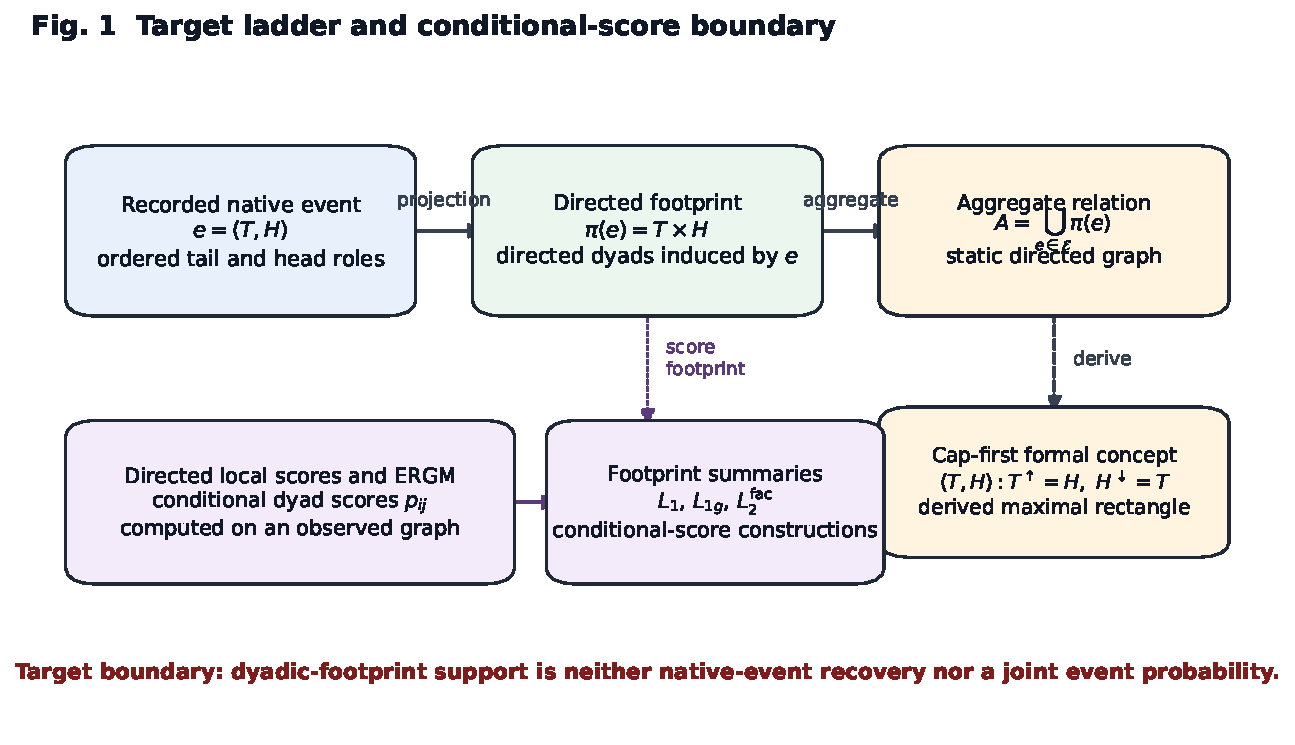
\includegraphics[width=\textwidth]{Fig1_target_ladder.pdf}
\caption{Target ladder and score map. The directed dyadic relation, cap-first formal concepts, and native ordered tail/head events are distinct objects. Projection and algebraic closure are not inverse reconstruction procedures. Conditional ERGM and lifted local scores concern candidate footprints; they do not by themselves define probabilities of recorded group events.}
\label{fig:ladder}
\end{figure}

\subsection{Directed formal context and cap-first concepts}
We construct a formal context $\mathbb K=(V_{\mathrm{out}},V_{\mathrm{in}},I)$ from the directed relation, using separate tail and head copies of $V$. Incidence $uIv$ holds exactly when $y_{uv}=1$. This object--attribute mapping is an analysis choice, rather than a claim that a graph arrives with a canonical event decomposition. For $X\subseteq V_{\mathrm{out}}$ and $Z\subseteq V_{\mathrm{in}}$, define
\begin{align}
X^{\uparrow}&=\{v\in V_{\mathrm{in}}:uIv\ \text{for every }u\in X\},\\
Z^{\downarrow}&=\{u\in V_{\mathrm{out}}:uIv\ \text{for every }v\in Z\}.
\label{eq:galois}
\end{align}
The operators reverse inclusion and satisfy $X\subseteq Z^{\downarrow}$ if and only if $Z\subseteq X^{\uparrow}$. The double derivations are extensive, monotone, idempotent closure operators. A formal concept is a pair $(T,H)$ satisfying $T^{\uparrow}=H$ and $H^{\downarrow}=T$ \citep{ganterWille1999}.

For a nonempty concept, every tail is incident to every head, and neither role can be enlarged without losing that complete rectangle. Under the bipartite-copy representation this is a maximal biclique, providing the graph-theoretic bridge to formal concepts \citep{zhangEtAl2014}. Maximality is inclusion-maximality, not a maximum-size optimization. Because the directed graph is loopless, an actor cannot occupy both roles of a nonempty complete rectangle: its diagonal incidence would then be required. Distinct copies of the actor set make the context formally bipartite, while the no-loop condition supplies the substantive role-disjointness of emitted nonempty concepts.

The benchmark enumerates the capped section
\begin{equation}
\mathcal C_3(D)=\{(T,H):T^{\uparrow}=H,\ H^{\downarrow}=T,\ 1\le |T|\le3,\ 1\le |H|\le3\}.
\label{eq:cap}
\end{equation}
The cap is applied during enumeration. It does not mean truncating a larger extent or intent to three actors and calling the fragment a concept. Closure and maximality are checked in the original relation; a maximal pair whose closure exceeds the cap is outside the reported section. The section is therefore not the full concept lattice and need not cover all arcs. Reporting uncovered arcs and footprint overlap is preferable to implying exhaustive representation from a bounded enumeration.

A native event need not be maximal in the aggregate. In the three-actor example above, both singleton-recipient events contribute to the same larger rectangle; the graph's nonempty concept combines them. Additional senders with matching recipients can expand its tail further. Conversely, a recorded event may sit inside a rectangle whose closure exceeds the cap and leave no exact capped match. These possibilities explain why a legitimate concept target is derived rather than observed. They also explain why concept recovery under arc missingness and native-type recovery under event missingness must use different positive sets.

For fidelity, let $\mathcal E_3$ be the cap-eligible native type set, and compare it with $\mathcal C_3(D)$ using exact equality of both ordered sets. Define $q=|\mathcal E_3\cap\mathcal C_3(D)|$, concept precision $q/|\mathcal C_3(D)|$, and native-type recall $q/|\mathcal E_3|$. Separately let $F_E$ and $F_C$ be the respective unions of footprints. Their Jaccard is $|F_E\cap F_C|/|F_E\cup F_C|$, and the two directional coverage fractions divide the same intersection by $|F_E|$ and $|F_C|$. These denominators express different representation questions. Exact equality can be zero while the union footprints agree strongly; neither measure should replace the other.

\subsection{Local directed quantities and footprint lifting}
All local quantities are calculated in a split's observed projection. Define the out-neighbour and in-neighbour sets $N^+(i)=\{v:y_{iv}=1\}$ and $N^-(i)=\{v:y_{vi}=1\}$, with degrees $d_i^+=|N^+(i)|$ and $d_i^-=|N^-(i)|$. For a nonloop candidate $i\to j$, let
\begin{align}
C^{OI}_{ij}&=N^+(i)\cap N^-(j),&s^{OI}_{ij}&=|C^{OI}_{ij}|,\\
C^{OO}_{ij}&=N^+(i)\cap N^+(j),&s^{OO}_{ij}&=|C^{OO}_{ij}|,\\
C^{II}_{ij}&=N^-(i)\cap N^-(j),&s^{II}_{ij}&=|C^{II}_{ij}|.
\label{eq:cn}
\end{align}
OI counts directed two-path intermediates from $i$ to $j$; OO counts shared targets; II counts shared sources. The total common-neighbour score is their sum. Although OO and II individually are symmetric in the endpoint labels, OI is not generally symmetric. Retaining the components therefore makes orientation content visible rather than disguising it in a single undirected neighbourhood intersection.

We use an Adamic--Adar-style degree-aware construction with explicitly directed weighting. Write $w(d)=1/\log d$ for $d>1$ and $w(d)=0$ otherwise. The implemented components are
\begin{align}
a^{OI}_{ij}&=\sum_{v\in C^{OI}_{ij}}w(d_v^++d_v^-),\\
a^{OO}_{ij}&=\sum_{v\in C^{OO}_{ij}}w(d_v^-),\qquad
 a^{II}_{ij}=\sum_{v\in C^{II}_{ij}}w(d_v^+),\\
a^{\mathrm{total}}_{ij}&=a^{OI}_{ij}+a^{OO}_{ij}+a^{II}_{ij}.
\label{eq:aa}
\end{align}
The OI intermediary is discounted by total directed activity, a shared target by its incoming popularity, and a shared source by its outgoing broadcast activity. Thus the reported total does not weight every component by the same degree. The name identifies a family resemblance to degree-discounted local indices; it does not assert that an undirected Adamic--Adar score is inherently directed. Directional adaptation is part of the present specification, consistent with the need to distinguish directed paths and neighbourhood roles in link scoring \citep{luZhou2011}.

Two additional components are reverse-arc support $r_{ij}=y_{ji}$ and the directed degree product $b_{ij}=d_i^+d_j^-$. The former measures observed reciprocity, while the latter combines source activity and target popularity without requiring a particular common neighbour. We lift any dyadic score $s$ to an ordered event candidate by its arithmetic footprint mean,
\begin{equation}
S_s(e)=m(e)^{-1}\sum_{(i,j)\in\pi(e)}s_{ij}.
\label{eq:lift}
\end{equation}
This permits the same dyadic ingredients to rank candidates with multiple arcs. It is an uncalibrated summary, not a likelihood for the group. The descriptive already-observed-footprint baseline is $B(e)=\ind\{\pi(e)\subseteq A_{\mathrm{obs}}\}$; it measures projection survival rather than reconstructing the type.

A useful algebraic connection explains why local closure quantities are relevant ERGM comparators. Define the ordered transitive-triple statistic $g_{\mathrm{tr}}(y)=\sum_{a,b,c\ \mathrm{distinct}}y_{ab}y_{bc}y_{ac}$. Adding $i\to j$ changes this count through three positions: as the shortcut, first leg, or second leg. Those contributions are respectively $s^{OI}_{ij}$, $s^{OO}_{ij}$, and $s^{II}_{ij}$, evaluated with the candidate dyad toggled off. An edges-plus-transitive-triples conditional logit is therefore affine in their total. This identity is specific to that statistic and conditioning. It does not equate geometrically weighted closure with the unweighted count, nor does it make arithmetic and geometric event lifting identical.

\section{ERGM conditional benchmark}
\subsection{Exponential family, change statistics, and MPLE}
For the fixed actor universe, let $\mathcal Y$ be the set of loopless binary directed graphs. An ERGM with statistic vector $g:\mathcal Y\to\mathbb R^p$ and parameter $\theta\in\mathbb R^p$ has mass function
\begin{equation}
\Pr_\theta(Y=y)=\frac{\exp\{\theta^\top g(y)\}}{\kappa(\theta)},\qquad
\kappa(\theta)=\sum_{z\in\mathcal Y}\exp\{\theta^\top g(z)\}.
\label{eq:ergm}
\end{equation}
The normalising constant sums over whole graphs, not over candidate event types. This is a model on a dyadic relation even when its statistics capture dependence among several dyads. No timestamp, occurrence count, recipient-list likelihood, or answer-window likelihood enters equation~\eqref{eq:ergm}. Such information can define targets and masks without being represented by the fitted graph family.

For a dyad $i\to j$, write $y_{ij}^+$ and $y_{ij}^-$ for otherwise identical graphs with that dyad set to one and zero. The change statistic is $\Delta_{ij}g(y)=g(y_{ij}^+)-g(y_{ij}^-)$. Taking the ratio of their ERGM masses cancels the normalising constant and gives
\begin{equation}
\Pr_\theta(Y_{ij}=1\mid Y_{-ij}=y_{-ij})
=\logitinv\{\theta^\top\Delta_{ij}g(y)\}.
\label{eq:conditional}
\end{equation}
This single-dyad conditional expression is exact for the specified ERGM and fixed parameter \citep{wassermanPattison1996,krivitskyEtAl2011}. It is not a marginal obtained by integrating over all other unknown arcs. In a masked benchmark, those other dyads are supplied as the split's observed binary graph, so the conditioning includes its retained ties and its currently absent ties. A conditional calculation must not be described as if the unobserved network had been jointly completed.

For each split we estimate $\theta$ by maximizing the log pseudolikelihood
\begin{equation}
\ell_{\mathrm{PL}}(\theta;y)=\sum_{i\ne j}
\left[y_{ij}\theta^\top\Delta_{ij}g(y)
-\log\{1+\exp(\theta^\top\Delta_{ij}g(y))\}\right].
\label{eq:mple}
\end{equation}
This is the log of the product of all local conditional Bernoulli terms, and its logistic-regression form makes the change-statistic design explicit. When the graph model contains dependent terms, the product is not the joint likelihood in equation~\eqref{eq:ergm}. MPLE and maximum likelihood should therefore not be treated as interchangeable estimators \citep{vanDuijnEtAl2009}. The empirical purpose here is ranking from the fitted conditional score, not parameter inference under a successfully simulated joint network distribution.

Every native-event scoring fit uses only the corresponding observed projection. Full-network coefficients are not recycled across masks, and held-out arcs are not added before computing candidate change statistics. Each candidate dyad is scored against the same split basis while its own toggle is handled through equation~\eqref{eq:conditional}. This applies to footprint arcs that remain observed as well as those absent in the training projection. Observed footprint survival consequently contributes conditional information but does not automatically force a score of one. No absent dyad is assigned a latent completion sampled from a fitted network law in the primary branch.

A successful fit status establishes that the specified MPLE objective and conditional prediction call produced available output under the software contract. It is not an ERGM goodness-of-fit assessment, an MCMC convergence certificate, or a claim that the fitted coefficients consistently identify a generating mechanism. Conversely, a failed or nonfinite fit remains a visible failure for that model and split rather than being replaced by a full-data fit or a simpler specification. This separation between availability and adequacy is especially important when a complex directed model has a convenient local logit but a difficult global simulation problem.

\subsection{Directed structural model ladder}
The static ladder nests density, mutuality, degree structure, and orientation-specific closure. Its foundation follows the exponential-family graph framework, while fixed-decay weighted degree and shared-partner terms address structural configurations without reducing every directed triangle to a single label \citep{snijdersEtAl2006,robinsEtAl2009}. Let $E(y)=\sum_{i\ne j}y_{ij}$ and $R(y)=\sum_{i<j}y_{ij}y_{ji}$ count edges and mutual dyads. For $\alpha>0$, define the geometric weight
\begin{equation}
f_\alpha(k)=e^\alpha[1-(1-e^{-\alpha})^k],\qquad f_\alpha(0)=0.
\label{eq:geom}
\end{equation}
The geometrically weighted outgoing and incoming degree terms are $G^+(y)=\sum_i f_\alpha(d_i^+)$ and $G^-(y)=\sum_i f_\alpha(d_i^-)$. Their diminishing increments make the degree terms different from a linear sum of degrees, which would duplicate the edge count.

Directed edgewise shared-partner counts distinguish outgoing two-paths (OTP), outgoing shared partners (OSP), and incoming shared partners (ISP). For an existing arc $i\to j$, their counts are respectively $s^{OI}_{ij}$, $s^{OO}_{ij}$, and $s^{II}_{ij}$ from equation~\eqref{eq:cn}. Write
\begin{equation}
W_Q(y)=\sum_{i\ne j}y_{ij}f_\beta(s^Q_{ij}),\qquad
Q\in\{OI,OO,II\}.
\label{eq:gwesp}
\end{equation}
Then $W_{OI}$ is OTP closure, $W_{OO}$ is OSP shared-target closure, and $W_{II}$ is ISP shared-source closure. Their statistics count geometrically weighted partners on existing directed edges; a toggle can also alter shared-partner counts on other edges. They should not be equated mechanically with the corresponding local candidate count. Cyclic triples add the contrasting closed configuration $i\to j\to k\to i$, counted once per directed cycle through $C(y)=\frac13\sum_{i,j,k\ \mathrm{distinct}}y_{ij}y_{jk}y_{ki}$.

The nested statistic sets are
\begin{align}
\mathrm{M0}:&\ E; & \mathrm{M1}:&\ E,R;\\
\mathrm{M2}:&\ E,R,G^+,G^-; & \mathrm{M3}:&\ \mathrm{M2}+W_{OI};\\
\mathrm{M4}:&\ \mathrm{M3}+W_{OO}+W_{II}; & \mathrm{M4c}:&\ \mathrm{M4}+C.
\label{eq:ladder}
\end{align}
Degree and shared-partner decays are fixed at $\alpha=\beta=0.5$ in the plan-aligned implementation. The labels describe nested specifications, not successive evidence of improved fit. The native-event conditional-footprint branch fits M0, M1, M3, and M4c on each split; the intermediate M2 and M4 define the complete structural ladder and its feasibility checks. M4c retains the cycle extension, but its reporting does not assert that cyclic structure has earned an incremental benefit over every preceding model.

With only edges, equation~\eqref{eq:conditional} is constant across candidate dyads. M1 adds the observed reverse arc to the conditional log-odds, making its connection to the reverse-arc heuristic transparent. M3 and M4c additionally allow degree and directed closure information to alter the local score. Such coherence is useful for implementation checking. It is not independent corroboration of a substantive reciprocity mechanism when two rankings use the same graph feature. The predeclared main contrast compares the M4c geometric summary with the M0 arithmetic reference; it does not isolate the contribution of the final cycle term.

\subsection{Footprint summaries and the joint-probability boundary}
For fitted single-dyad conditional scores $p_{ij}$ and $m=m(e)$, define
\begin{align}
L_1(e)&=m^{-1}\sum_{(i,j)\in\pi(e)}p_{ij},\\
L_{1g}(e)&=\exp\left[m^{-1}\sum_{(i,j)\in\pi(e)}\log p_{ij}\right],\\
L_2^{\mathrm{fac}}(e)&=\prod_{(i,j)\in\pi(e)}p_{ij}.
\label{eq:Ls}
\end{align}
The arithmetic mean summarizes average support; the geometric mean responds more strongly to a weakly supported arc while normalizing by footprint size. The factorized product compounds the individual scores and is evaluated on the log scale for numerical stability. At fixed arity its ranking agrees with the geometric mean because $L_2^{\mathrm{fac}}=L_{1g}^{m}$. Across arities, that exponent varies, so the product introduces a footprint-size effect. Arity matching prevents positive and negative candidates from differing in size within their matched comparisons, but it does not make all candidate footprints globally equal in size.

None of these summaries is a jointly simulated or matched-marginal quantity. To articulate the distinction, let $F=\pi(e)$ and let $O_e$ be one common observation constraint for all unknown dyads in $F$. A matched-marginal product would use $\prod_{(i,j)\in F}\Pr(Y_{ij}=1\mid O_e)$; a joint footprint probability would use $\Pr(Y_{ij}=1\ \forall(i,j)\in F\mid O_e)$. The former need not equal the latter under dependence. More fundamentally, neither is the primary product in equation~\eqref{eq:Ls}: its individual factors condition on the other dyads supplied by the observed training graph, rather than integrate them under the same candidate-wide completion constraint.

Even a valid joint footprint probability would remain a probability of a graph configuration, not of the native event record. Multiple record collections can generate the same complete footprint, as the non-identifiability example shows. For a formal concept, completeness alone would also omit the maximality requirement. These distinctions are why we label the primary quantities conditional-pseudolikelihood footprint scores. The Enron higher-order MCMC feasibility gate did not pass, so no primary jointly simulated dependence increment is reported. A bounded MPLE parameter-plug-in simulation is only a supplementary score-mechanics sensitivity and cannot substitute for successful higher-order MCMC likelihood estimation.

\section{Data and missingness design}
\subsection{Source construction and target eligibility}
Table~\ref{tab:eligibility} states eligibility before performance. The two primary event-type experiments use fixed 100-actor cores: strict Enron internal-custodian records and reconstructed MathOverflow answer-window events. EU-core and CAVIAR contribute only restricted dyadic or representation evidence, not additional primary native-event replications. Eligibility is target-specific. A source can support a static directed relation without supporting a group record, and a chronologically indexed dyadic source does not automatically identify simultaneous multi-recipient events. Accordingly, we do not manufacture native types from coincident timestamps or from a matrix's complete rectangles.

\begin{table}[t]
\centering
\caption{Dataset and target eligibility. ``Primary'' refers to the event-first native-type benchmark, not to a population sample. Concept targets are derived; restricted dyadic evidence does not supply native groups. Blocked or pending sources contribute no substantive result.}
\label{tab:eligibility}
\small
\begin{tabular}{@{}P{0.19\textwidth}P{0.22\textwidth}P{0.51\textwidth}@{}}
\toprule
Source & Admitted scope & Construction or restriction\\
\midrule
Enron strict core & Primary native types; footprints, concepts, roles & Complete approved internal sender--To/Cc heads; 1998--2002. Monthly dyadic diagnostic only.\\
MathOverflow core & Primary reconstructed native types; footprints, concepts, roles & Distinct eligible answerers $\to$ asker within 30 days; all participants in fixed core. No chronological pilot.\\
EU-core & Restricted directed dyadic and concept evidence & No primary native-event construction. Bounded 30-day dyadic chronology; concept section exploratory.\\
CAVIAR full matrix & Restricted static dyadic/footprint evidence & Approved caller-to-receiver orientation of the unique-labelled full matrix. Phase series excluded.\\
Ciel & Blocked & Source-specific row/column communication orientation unresolved.\\
Jmail v1 & Audit only; admissibility pending & Source-stream, entity-resolution, and recipient-policy gates unresolved.\\
\bottomrule
\end{tabular}
\end{table}

The Enron source is the official CMU distribution dated 7 May 2015, maintained by Cohen. Its provenance runs through publicly released FERC material and the CALO preparation documented by the official dataset record \citep{cohen2015}. That release is not an uncensored organizational census: its documentation notes redactions, omitted attachments, and corrections. Our benchmark adds a stricter internal identity and complete-head boundary. It should therefore be understood as a conservative retained-record experiment, not as reconstruction of the full Enron communication system or its real missing-data process.

The approved custodian mapping automatically accepts a unique rank-one sent-folder address candidate only with at least 90\% support and no sharing of that top-ranked address across custodians. This yields 110 approved identities. A retained record must have a mapped sender and mapped identities for every To/Cc recipient. If any participant is unmapped, the entire record is excluded rather than retaining a clipped internal recipient subset. A recipient mapping to the sender's own custodian is removed, and the resulting event must remain nonempty and loopless. Distinct maildir records are retained after raw-content and message-identifier duplicate audits; recurrence is subsequently represented by occurrence counts when identical ordered types are grouped.

The temporal policy retains the inclusive UTC interval from the start of 1998 to the end of 2002. It removes isolated out-of-period timestamps rather than interpreting them as a contiguous extension of the observation window. The strict projection contains 7,881 complete records among the approved identities. A deterministic sent-plus-received activity ranking fixes the primary 100-actor core; requiring all participants to belong to that core retains 7,820 native records and 635 static directed arcs. The graph has 9,900 possible nonloop dyads, so the retained relation is sparse but not an empty structural screen. These counts describe the selected core, not all available source emails.

The complete-head rule is substantively consequential. A permissive rule could retain more internal dyads by discarding unmapped recipients, but it would alter the group label and turn native email heads into censored projections. The strict rule instead trades breadth for a defensible statement that every retained head is complete within the approved identity policy. Its severe selection loss is thus an explicit boundary, not evidence that omitted contacts did not occur. Applying the arity cap to the core retains 7,793 of its 7,820 records, grouped into 719 event types. The cap has small record loss in this selected Enron core, but that observation does not validate the cap for an unrestricted email population.

MathOverflow uses the public Stack Exchange data-dump snapshot dated 7 April 2024, rather than substituting a derived temporal-edge release for the raw post reconstruction \citep{mathoverflow2024}. The official data-dump access page identifies the public distribution route; the archived snapshot identifies the source used here. Questions and answers are related through their retained parent and owner fields. For each eligible question, the analyst-defined event is the set of distinct eligible answerers appearing within 30 calendar days of the question's creation, directed toward its asker. Comments, ownerless or anonymous users, and self-answers are excluded. Multiple answers by the same user to the same question collapse to one answerer contribution.

The reconstruction policy follows a descriptive latency and eligibility profile, not a claim that all answers within a month formed one simultaneous interaction. The first-distinct-answerer latency distribution has a material long tail. Thirty days retains short-to-medium response coverage without pooling years-late answers into the same group. Seven- and 90-day windows are declared bounded construction sensitivities; the 365-day profile remains descriptive. The primary build yields 91,161 reconstructed events on the public rows. Its full projection has 32,117 participants, and deterministic activity selection fixes the 100-actor core. Requiring every answerer and the asker to remain in the core retains 1,949 reconstructed events and 1,020 static directed arcs; its cap-eligible section has 1,071 ordered types.

These answerer-to-asker groups are not directly recorded multi-recipient communication events. Their grouping depends on the chosen response window and duplicate-answerer policy, and their orientation represents contribution toward a question asker. Calling them reconstructed native types keeps the benchmark's event layer distinct from concepts derived later from the graph, without denying the analyst's role in defining it. The opposite singleton-role patterns in Enron and MathOverflow are useful design contrasts, but source and core selection confound any simple attribution of their performance differences to role arity alone.

EU-core supplies a fixed directed dyadic core and a bounded chronological diagnostic. Its cap-three concept section is small and low-coverage relative to Enron, so it is restricted to exploratory representation claims with explicit candidates. It is not promoted to a primary source of native groups. CAVIAR's approved full matrix has a source-supported caller-to-receiver interpretation, while its phase series remains excluded because an unresolved duplicate actor label prevents a reliable temporal entity map. A static relation can therefore be admitted while chronology remains inadmissible. Neither restricted source is counted as another independent network replication of the native-event result.

Ciel remains blocked by unresolved source-specific communication orientation, and Jmail remains audit-only pending source-stream, identity, and recipient-policy decisions. Structural usability or available headers alone do not resolve those gates. We report their status to distinguish exclusion from an adverse performance outcome, but show no substantive prediction values for them. Manuscript tables use aggregate-safe summaries only. Source archives, message bodies, actor-address maps, raw records, full candidate panels, and candidate-level predictions are excluded from manuscript outputs and from the repository's tracked research evidence.

\subsection{Event-first type withholding}
For each primary core, define $\mathcal E_3$ from all cap-eligible types and retain occurrence counts $c_e$. A mask $M\subset\mathcal E_3$ withholds every record of each selected type. The observed type set is $\mathcal E_{\mathrm{obs}}=\mathcal E_3\setminus M$, and the training arc set is $A_{\mathrm{obs}}=\bigcup_{e\in\mathcal E_{\mathrm{obs}}}\pi(e)$. The reference full projection for masking is the cap-restricted union $A_3=\bigcup_{e\in\mathcal E_3}\pi(e)$, not a graph silently augmented with out-of-cap records. This ordering makes type labels the experimental units and prevents recurrence from leaking an identical held-out type through an observed copy.

Under MCAR, we uniformly sample without replacement exactly $\lfloor0.30|\mathcal E_3|\rfloor$ types. Every subset of that size has the same selection probability. This fixed-count design has dependent selection indicators within a mask, even though selection is unrelated to type activity. Under MNAR-out, define full-data outgoing role activity
\begin{equation}
a_v^{\mathrm{out}}=\sum_{e\in\mathcal E_3}c_e|H_e|\ind\{v\in T_e\},\qquad
w_e=|T_e|^{-1}\sum_{v\in T_e}a_v^{\mathrm{out}}.
\label{eq:activity}
\end{equation}
Independently include type $e$ in the withheld set with probability $q_e=\min(1,\lambda w_e)$, choosing $\lambda$ so that $\sum_e q_e=0.30|\mathcal E_3|$. In Enron the tail is a singleton sender; in reconstructed MathOverflow the average spans its distinct answerer tail. The expected type rate is fixed, but the realized number withheld can vary. Saturation at one is part of the predeclared rule.

MNAR-out is manuscript shorthand for this full-data, role-activity-dependent omission design. The oracle uses the complete cap-eligible records to define the stress test, including information unavailable after masking. It is not an empirical diagnosis that either corpus is MNAR, nor an identified model of its original collection process. Rubin's missingness framework motivates explicitly stating that dependence \citep{rubin1976}; the operational mask is our simulation choice. No oracle activity is supplied to the predictor. We keep 30 fixed masks per mechanism and dataset, with all methods using the same corresponding training graph and candidate panels.

Three severities must be distinguished: $\rho_{\mathrm{type}}=|M|/|\mathcal E_3|$, $\rho_{\mathrm{record}}=\sum_{e\in M}c_e/\sum_{e\in\mathcal E_3}c_e$, and $\rho_{\mathrm{arc}}=|A_3\setminus A_{\mathrm{obs}}|/|A_3|$. A high-frequency type increases record loss, while shared arcs can survive its removal. Likewise, the complete-footprint survival fraction averages $B(e)$ over held-out types. These quantities need not move together, so nominal 30\% type withholding cannot be interpreted as 30\% arc loss or equal severity across mechanisms. Realized-rate and removal-stratum accounting is retained with the masks; the performance summaries below do not replace it with one universal severity number.

The formal-concept recovery branch uses a separate arc-first design: remove unique arcs and ask which full-relation capped concepts are lost from the re-enumerated observed section. Random, observed-degree-matched, and non-maximal-complete non-concept panels remain separate structural evaluations. This distinction matters because deleting arcs can destroy maximal rectangles without withholding an identifiable record type, and withholding a type can leave a complete rectangle intact. Supplementary footprint-free concept stress tests deliberately remove whole selected footprints. Neither that stronger stress regime nor the focused mask-rate and MNAR-in sensitivities changes the primary event-first design or its target definition.

\section{Evaluation and within-network uncertainty}
\subsection{Random, hard, and role-assignment competitions}
The random native-type panel combines held-out positives with one sampled non-event negative per eligible positive, matched exactly on tail and head arity. Negatives must be absent from the entire cap-eligible native-type set, excluding both observed and held-out types. This full-type exclusion is used only to establish benchmark labels; it does not provide features to the predictor. Candidate participants must be pairwise within weak distance two in the split's observed projection. Weak distance ignores orientation for locality screening, while the actual score retains direction. The eligibility rule therefore defines a local competition set rather than an unrestricted search over all actor subsets.

Some held-out types can fall outside that observed local universe. Their exclusion is recorded as candidate coverage, not concealed by replacement positives or relabelling them as negatives. The random-panel estimand is ranking among eligible held-out types and arity-matched non-types under this rule. It is not recall over every possible missing group. Likewise, a negative is a non-type under the frozen source construction, not proof that the actors could never interact together. This distinction is particularly important for MathOverflow, where another answer window could change the reconstructed label while leaving the same actors available.

The reversal/orientation panel contrasts a held-out $e=(T,H)$ with $(H,T)$ only if the reversal is an unseen type and both candidates satisfy the split-specific locality contract. Reversal preserves participants and footprint size, but swaps the two role arities when they differ. The role-exchange panel swaps one tail actor and one head actor, preserving the participant set and each role's arity. It also requires the transformed group to be unseen and locally eligible. These panels are separately balanced contrasts on selected subsets of the held-out target. No unavailable reversal or exchange is filled with an easier random alternative. Their coverage and exclusions belong to the task description, so differences from random-panel values cannot be read as a controlled effect of difficulty alone.

Fixed-role assignment asks a third question. Given $U=T\cup H$ and the true arities $(t,h)$, enumerate every compatible partition $(T',U\setminus T')$ with $|T'|=t$. There are $\binom{t+h}{t}$ possibilities. The score uses only the observed graph, but the evaluator supplies the participant set and arities. This deliberately removes actor-set retrieval from the task. Every held-out type is evaluated in this branch, rather than restricting the task to the random panel's eligible positives. Top-one success measures assignment among known participants; it does not demonstrate identification of participants that were not supplied.

Ties are resolved by expectation under uniform ordering of the tied partitions. If $a$ alternatives score strictly above the correct partition and $b$ tie with it, expected top-one accuracy is $\ind\{a=0\}/b$, and expected reciprocal rank is $b^{-1}\sum_{r=a+1}^{a+b}r^{-1}$. A constant-score baseline consequently depends on partition count, unlike the constant baseline in a balanced binary panel. The reported overall top-one accuracy weights the arity strata by their event evaluations across masks. Repeated evaluations of the same underlying type under different masks are not new source events or independent networks.

\subsection{Ranking metrics and their denominators}
Native-type footprint scores are evaluated through rankings, not a universal threshold. For a candidate panel, precision at a cutoff is the positive fraction among selected candidates, and recall is the selected fraction of panel positives. ROC-AUC is the probability that a randomly chosen positive outranks a randomly chosen negative, with half credit for ties. PR-AUC uses the project's tie-aware average-precision convention: sum precision at each distinct-score block times its increase in recall. This convention is a stepwise precision--recall area, not an unspecified trapezoidal interpolation. Precision and recall at $k$ are also available, with $k$ equal to the number of positives in the balanced retrieval panel.

Precision--recall summaries are relevant when the full group-candidate space is highly imbalanced, and their dependence on prevalence must be respected \citep{saitoRehmsmeier2015}. Here the scored panels deliberately impose one positive per negative. Their PR-AUC is therefore a defined case-control panel quantity; neither it nor a footprint score estimates the probability of an event at natural prevalence. A constant ranking yields average precision 0.5 in these panels. The fixed-role competition has no comparable binary prevalence and is evaluated separately. We do not report accuracy, F1, or log loss for the uncalibrated native-type scores as if they came from an event-probability model.

\subsection{Paired whole-mask comparison}
For dataset $d$ and mechanism $m$, let $Q_{r,A}$ and $Q_{r,B}$ be two methods' PR-AUC values on the same frozen mask $r$, including the same training graph and candidate panel. With $R=30$, the paired difference is $D_r=Q_{r,A}-Q_{r,B}$ and the reported effect is $\bar D=R^{-1}\sum_rD_r$. The main contrast fixes $A$ as M4c with $L_{1g}$ and $B$ as M0 with $L_1$. It is selected because its density reference was predeclared, not because it maximizes an inspected table. Other score contrasts remain exploratory unless a separate multiplicity policy is specified.

A percentile bootstrap resamples 30 whole-mask indices with replacement and recomputes the mean paired difference in each of 10,000 draws. Its 2.5th and 97.5th percentiles define the reported 95\% interval. The resampling unit is neither a candidate nor a dyad. Holding the paired methods together preserves each split's shared difficulty and avoids treating dependent arcs within a footprint as separate experimental replications. The bootstrap rationale follows standard resampling principles \citep{efronTibshirani1994}; matched-system evaluation motivates preserving shared units when resampling complex metrics \citep{bergKirkpatrickEtAl2012}. Those general principles do not transform masks into a network population sample.

The paired sign-flip procedure assigns independent signs $s_r\in\{-1,+1\}$ to the 30 differences in each of 20,000 Monte Carlo draws and compares $|R^{-1}\sum_rs_rD_r|$ with $|\bar D|$. With $b$ draws at least as extreme, the reported value is $(b+1)/(20{,}000+1)$. Its smallest attainable value is $1/20{,}001$, approximately 0.00005, not zero. This is a two-sided paired reference calculation under sign exchangeability of differences about the null; it is not a general permutation license for graph-dependent candidate labels. Fixed seeds preserve reproducibility, not an empirical proof of the reference assumptions.

The inferential boundary is explicitly within a fixed network, source construction, masking mechanism, and candidate rule. The 30 masks expose repeated missingness realizations of the same graph; they do not supply 30 independent organizations or communities. Bootstrap intervals characterize the generated-mask distribution, and sign-flip values summarize the paired reference evidence for the specified contrast. We do not pool masks across datasets, infer a cross-network mean, or compare the two effects as if their intervals came from representative network samples. The four primary cells are reported separately even when their signs agree.

\subsection{Bounded chronological MPLE check}
The chronological module uses three consecutive retained panels, giving two response transitions in Enron and EU-core. It distinguishes factorized lagged scores from specifications containing contemporaneous response-network statistics. For a history-only logistic specification with fixed features $x_{ij}(Y_{t-1})$, the chosen model factorizes as a product of Bernoulli terms conditional on history. This factorization is a property of the specification, not a claim that observed temporal networks are independent. Adding statistics of $Y_t$ instead yields a conditional graph framework in which within-window configuration can enter a dyad's score, a distinction consistent with temporal exponential-family modeling \citep{hannekeEtAl2010}.

Three lagged-score models and a small btergm MPLE ladder supply a numerical status check. The implementation uses bootstrapped pseudolikelihood, not MCMC likelihood estimation \citep{leifeldEtAl2018}. Its labels are $T_{\mathrm{tt}}$ for edges plus lagged total common neighbours; $T0$ for edges, contemporaneous mutuality, autoregressive and delayed reciprocity terms, lagged OI/OO/II, and lagged endpoint degrees; $T1$ adds current weighted degrees; $T2$ adds current OTP/OSP/ISP closure; and $T2_{-H}$ removes explicit history terms from that structural specification. Thus not every model with a lagged component is history-only. The module uses only 20 temporal bootstrap replications. It records availability over the two transitions and supplies no out-of-time ranking contest, native-event forecast metric, or jointly simulated temporal result.

\section{Results}
\subsection{Representation fidelity is not event recovery}
The two primary cores support substantial but different capped concept sections. Table~\ref{tab:fidelity} reports 232 concepts in Enron and 207 in MathOverflow, against 719 and 1,071 cap-eligible native types respectively. Their counts are not directly comparable measures of group richness: they depend on each aggregate relation and on the same bounded closure rule. More decisively, exact equality of ordered tail/head sets is absent in both cores. Concept precision and native-type recall are zero, even though every emitted object satisfies the formal-concept definition. These are representation-audit results, not false-negative rates of a trained event predictor.

\begin{table}[t]
\centering
\caption{Cap-first concept/native-type fidelity on the fixed cores. Both role caps are three. Precision and recall use exact ordered tail/head equality; all footprint fractions compare unions of directed arcs. Values are descriptive representation diagnostics, not predictive scores.}
\label{tab:fidelity}
\small
\begin{tabular}{@{}lrr@{}}
\toprule
Quantity & Enron & MathOverflow\\
\midrule
Actors & 100 & 100\\
Static arcs & 635 & 1,020\\
Cap-eligible native types & 719 & 1,071\\
Capped formal concepts & 232 & 207\\
Exact ordered-set matches & 0 & 0\\
Concept precision & 0.0000 & 0.0000\\
Native-type recall & 0.0000 & 0.0000\\
Footprint Jaccard & 0.8567 & 0.6634\\
Native footprint covered by concepts & 0.8662 & 0.6647\\
Concept footprint covered by native types & 0.9873 & 0.9970\\
\bottomrule
\end{tabular}
\end{table}


Fig.~\ref{fig:fidelity} shows why the exact and footprint measures should be considered together. Footprint Jaccard is 0.8567 in Enron and 0.6634 in MathOverflow. Concepts cover 86.62\% of the capped native footprint arcs in Enron, while native footprints cover 98.73\% of concept arcs; the corresponding MathOverflow coverage fractions are 66.47\% and 99.70\%. The strong asymmetry means the capped concept section largely lies within event-derived dyadic support but does not exhaust that support. It does not mean the concept set nearly recovers the event set. High union overlap is compatible with the complete absence of exact ordered-group matches.

\begin{figure}[t]
\centering
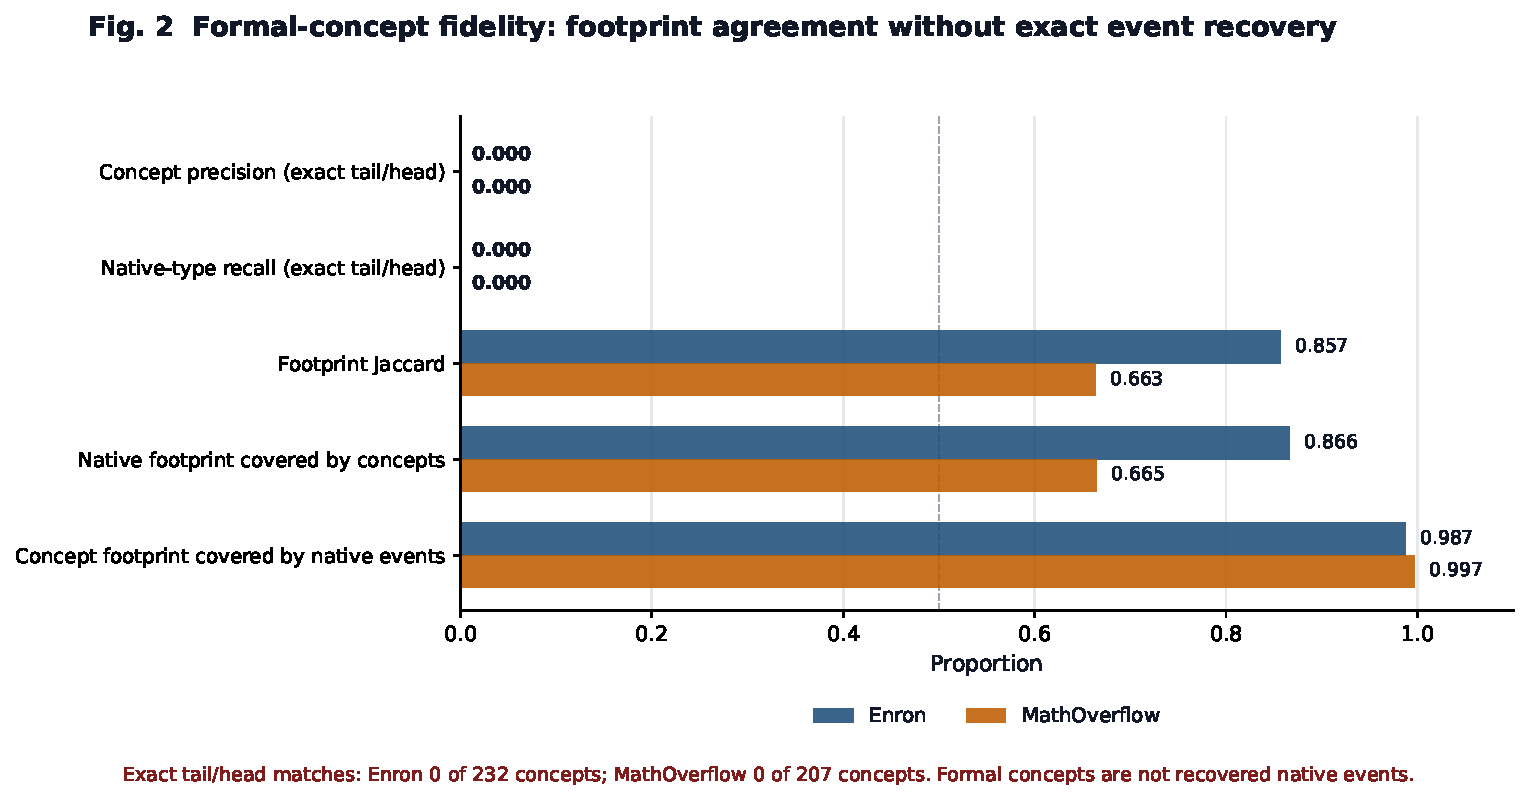
\includegraphics[width=\textwidth]{Fig2_concept_event_fidelity.pdf}
\caption{Formal-concept/native-type fidelity in the fixed primary cores under tail and head caps of three. Exact precision and recall are zero in both datasets despite substantial dyadic footprint overlap. Jaccard and the two coverage fractions compare unions of arcs, not record-level or event-type recovery.}
\label{fig:fidelity}
\end{figure}

The Enron audit further finds that each capped concept has at least two contributing recorded types, reinforcing its interpretation as an aggregate rectangle assembled across records. The result is not merely that concepts are noisy email groups. They answer a different structural question. Nor does zero equality prove that exact event--concept equality is impossible in every graph: the construction in Section~2 demonstrates non-invertibility generically, while the audit establishes absence of exact matches for these two selected cores. A degree-preserving rewiring comparison is retained as a supplementary representation diagnostic, not as another predictive benchmark. It does not change the fact that exact recovery is absent in the observed section.

\subsection{Random-panel conditional footprint discrimination}
Table~\ref{tab:native} combines the three primary evaluations while keeping their metrics distinct. Panel A reports means and mask standard deviations over 30 frozen masks in each dataset--mechanism cell. The M0 arithmetic reference has PR-AUC 0.5000 throughout because its constant conditional dyad score remains constant after averaging over any footprint. M4c with geometric lifting reaches 0.8584 and 0.8324 in Enron under MCAR and MNAR-out, and 0.7396 and 0.7394 in MathOverflow. These values support substantial random-panel discrimination relative to density alone. They do not identify a probability of the native group or isolate the effect of cycles.

\begin{table}[p]
\centering
\caption{Primary native-type evaluations in one table with distinct tasks. Panels A and B show PR-AUC mean (mask SD), each from 30 completed masks per cell; PR-AUC is tie-aware average precision on a separate balanced panel. Panel C shows event-evaluation-weighted, uniform-tie-aware top-one role accuracy, not PR-AUC. Selected score rows are predeclared summaries, not an overall winner selection.}
\label{tab:native}
\small
\setlength{\tabcolsep}{4pt}
\begin{tabular}{@{}lrrrr@{}}
\toprule
 & \multicolumn{2}{c}{Enron} & \multicolumn{2}{c}{MathOverflow}\\
\cmidrule(lr){2-3}\cmidrule(l){4-5}
Score & MCAR & MNAR-out & MCAR & MNAR-out\\
\midrule
\multicolumn{5}{l}{\textbf{Panel A. Random arity-matched native-type ranking}}\\
Already-observed footprint & 0.6279 (0.0220) & 0.5816 (0.0175) & 0.6050 (0.0113) & 0.6071 (0.0176)\\
Directed AA total & 0.7966 (0.0187) & 0.7472 (0.0206) & 0.7589 (0.0237) & 0.7593 (0.0218)\\
Reverse-arc mean & 0.7501 (0.0186) & 0.7761 (0.0177) & 0.5207 (0.0092) & 0.5219 (0.0108)\\
M0::$L_1$ & 0.5000 (0.0000) & 0.5000 (0.0000) & 0.5000 (0.0000) & 0.5000 (0.0000)\\
M4c::$L_{1g}$ & 0.8584 (0.0183) & 0.8324 (0.0158) & 0.7396 (0.0257) & 0.7394 (0.0258)\\
\addlinespace
\multicolumn{5}{l}{\textbf{Panel B. Directed hard-panel native-type ranking}}\\
\multicolumn{5}{l}{\emph{Reversal/orientation}}\\
Directed AA total & 0.5177 (0.0118) & 0.4792 (0.0099) & 0.6060 (0.0095) & 0.5938 (0.0104)\\
Reverse-arc mean & 0.4784 (0.0144) & 0.5685 (0.0233) & 0.4661 (0.0024) & 0.4621 (0.0027)\\
M0::$L_1$ & 0.5000 (0.0000) & 0.5000 (0.0000) & 0.5000 (0.0000) & 0.5000 (0.0000)\\
M4c::$L_{1g}$ & 0.4899 (0.0194) & 0.5575 (0.0250) & 0.6543 (0.0234) & 0.6283 (0.0199)\\
\addlinespace
\multicolumn{5}{l}{\emph{Role exchange}}\\
Directed AA total & 0.5197 (0.0160) & 0.4890 (0.0131) & 0.6094 (0.0133) & 0.6104 (0.0133)\\
Reverse-arc mean & 0.4781 (0.0100) & 0.5515 (0.0173) & 0.4688 (0.0024) & 0.4661 (0.0026)\\
M0::$L_1$ & 0.5000 (0.0000) & 0.5000 (0.0000) & 0.5000 (0.0000) & 0.5000 (0.0000)\\
M4c::$L_{1g}$ & 0.4969 (0.0202) & 0.5423 (0.0203) & 0.6326 (0.0255) & 0.6115 (0.0198)\\
\addlinespace
\multicolumn{5}{l}{\textbf{Panel C. Fixed-participant, fixed-arity role assignment}}\\
Already-observed footprint & 0.3377 & 0.2722 & 0.5257 & 0.5267\\
Degree-product mean & 0.4478 & 0.3010 & 0.7817 & 0.7521\\
Directed AA total & 0.4832 & 0.3851 & 0.6972 & 0.6831\\
Reverse-arc mean & 0.6012 & 0.6541 & 0.3907 & 0.3753\\
Event evaluations & 6,450 & 6,449 & 9,630 & 9,626\\
\bottomrule
\end{tabular}
\par\vspace{4pt}
\begin{minipage}{\textwidth}\footnotesize
AA denotes the directed Adamic--Adar-style score of equation~\eqref{eq:aa}. The already-observed footprint is a descriptive survival baseline. Hard panels include only valid unseen transformed alternatives; unavailable pairs are not replaced by random negatives. Panel C counts repeated type evaluations over masks and weights the fixed arity strata accordingly. The same underlying types can appear under several masks; counts are not independent source records. Full coverage and arity accounting are retained with the aggregate audit records, rather than inferred from PR-AUC.
\end{minipage}
\end{table}


The local-score profiles provide a substantive qualification to that reference comparison. Enron's total directed Adamic--Adar score is stronger than its reverse-arc mean under MCAR, while reverse-arc support is stronger under the activity-biased stress design. MathOverflow's total directed Adamic--Adar score is informative in both mechanisms, whereas reverse arcs are near the balanced-panel baseline. The displayed M4c geometric score does not exceed that heuristic in MathOverflow's random panels. Thus the predeclared ERGM--density improvement is not a claim of general superiority over local scores. Selecting a favourable dataset-specific winner would obscure both the reference definition and the change in feature ordering.

The already-observed-footprint indicator is also above the constant baseline in the random panels. That is expected when other retained event types preserve some held-out footprints. Its informative ranking is not identical-type leakage because all records of the held-out type were removed. Equally, its nontrivial score warns against interpreting a high random-panel value as completion of wholly unseen arc configurations. The primary task includes both partly missing and already-supported footprints. The supplementary footprint-free stress regime asks a different question and should not be silently substituted for this event-first experiment.

\subsection{Hard panels and role assignment change the claim}
Panel B preserves more participant and role structure than random negative sampling. In Enron, M4c geometric PR-AUC is 0.4899 for reversal and 0.4969 for role exchange under MCAR: random-panel discrimination does not persist in those transformed competitions. Under MNAR-out the same scores rise only modestly, to 0.5575 and 0.5423. Reverse-arc support changes from below the balanced reference under MCAR to positive separation under MNAR-out. These are descriptive mechanism-dependent patterns, not a demonstrated general reversal of causal reciprocity effects or evidence that a complex model consistently recovers sender roles.

MathOverflow has a different directed profile. Its M4c geometric score remains above the reference in both hard panels and mechanisms, ranging from 0.6115 to 0.6543, while reverse-arc scores are below the reference. The difference from Enron is useful precisely because it prevents a uniform narrative that all random-panel gains necessarily vanish or necessarily transfer. Fig.~\ref{fig:profiles} makes the panel-dependent levels visible. Its profile lines summarize means for the displayed conditional and heuristic families; they are not matched-mask confidence intervals or performance at a common natural prevalence. Hard-panel selection still restricts the subset to which each value applies.

\begin{figure}[t]
\centering
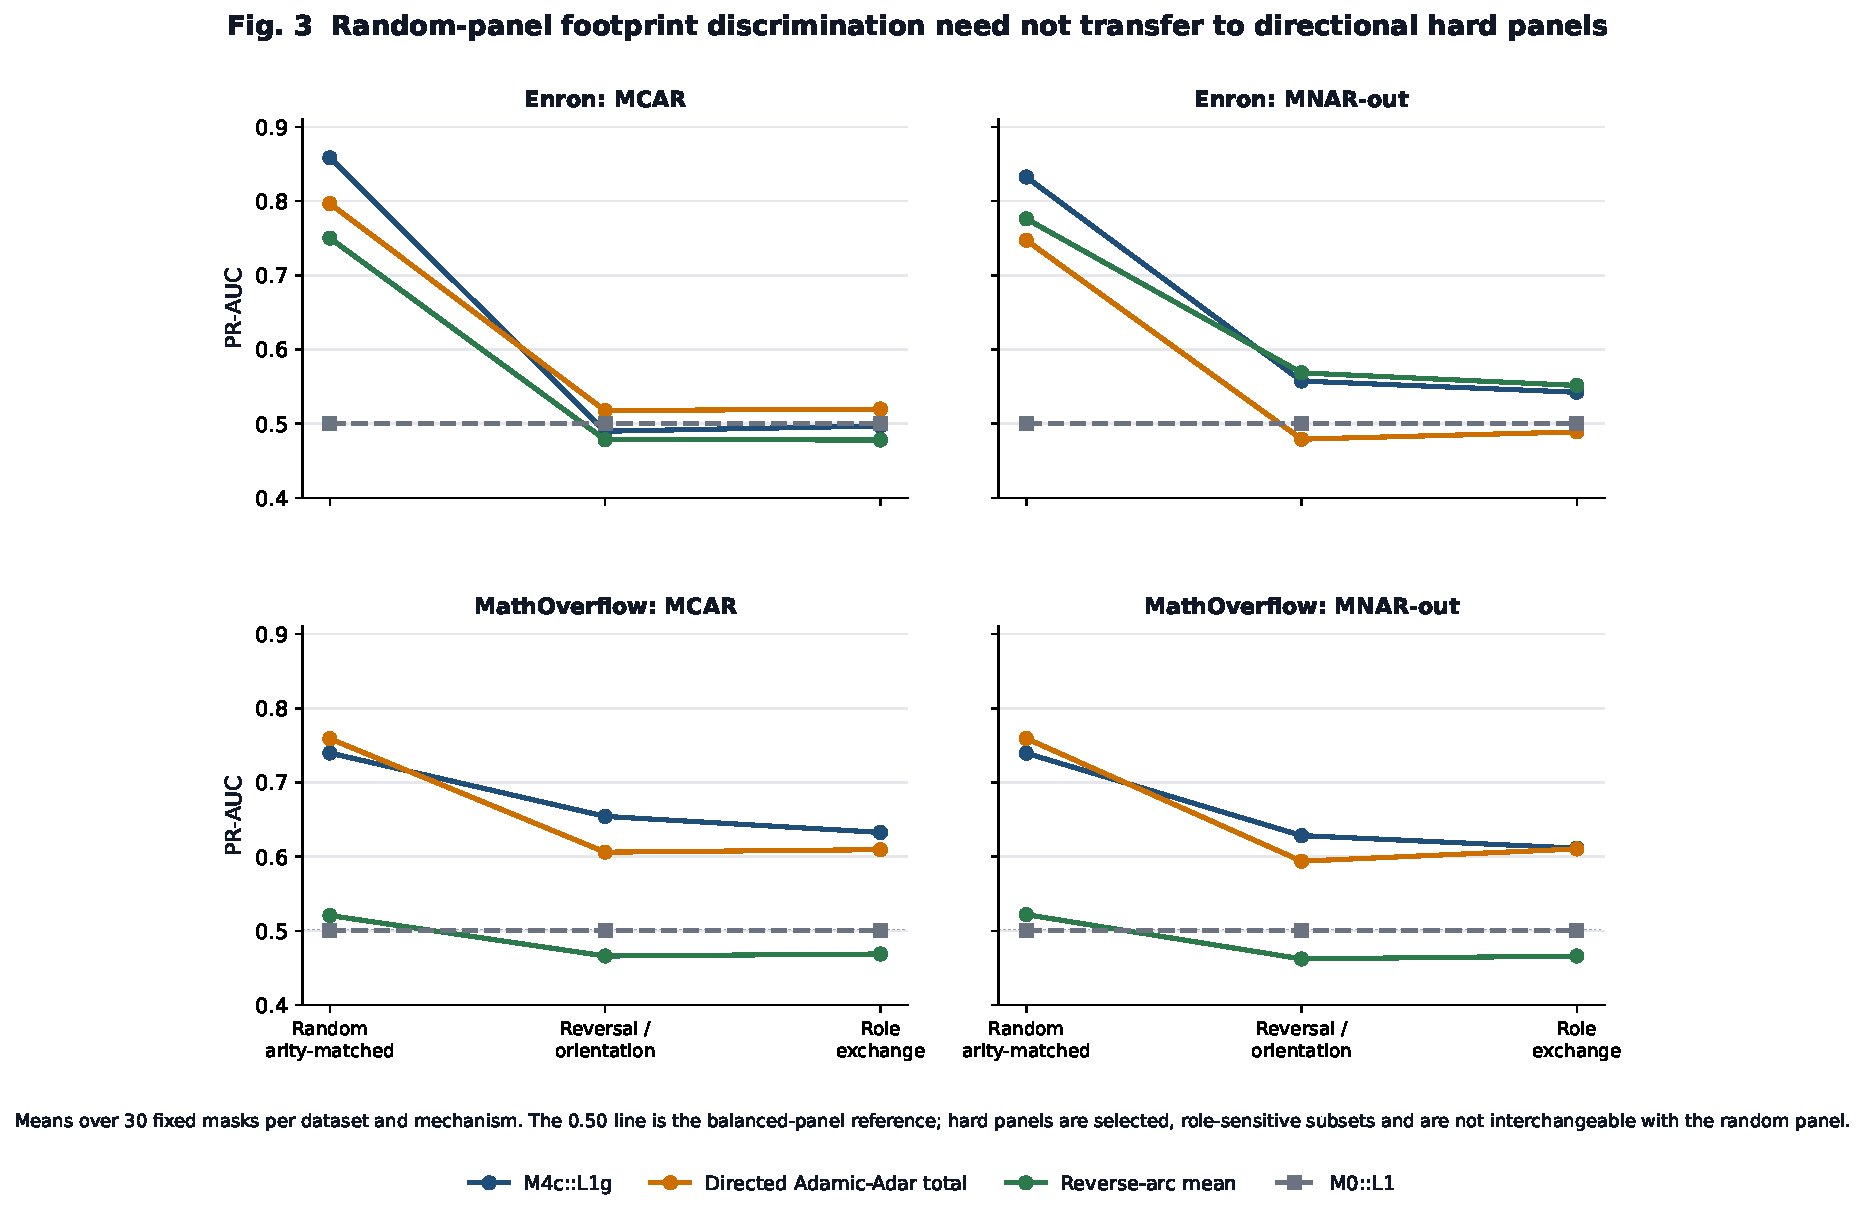
\includegraphics[width=\textwidth]{Fig3_primary_panel_profiles.pdf}
\caption{Primary panel profiles by fixed dataset and masking mechanism. Values summarize PR-AUC over 30 masks for random arity-matched, reversal/orientation, and role-exchange panels. The 0.5 line is the balanced constant-score reference. Profiles compare distinct selected competitions, not a universal event-prevalence scale; paired uncertainty is reported separately in Table~\ref{tab:paired}.}
\label{fig:profiles}
\end{figure}

Panel C conditions on the known participant set and role arities. Enron's reverse-arc mean yields weighted top-one accuracy 0.6012 under MCAR and 0.6541 under MNAR-out. MathOverflow is instead better ranked by the displayed degree-product mean, at 0.7817 and 0.7521. Those role accuracies are not PR-AUC values and have arity-dependent tie baselines. In particular, the event-evaluation counts accumulate repeated tests across masks rather than independent records. This branch shows that observed direction can carry assignment information after participants are supplied, but cannot establish retrieval of unknown actor sets. The displayed role comparison is heuristic; it is not an unreported ERGM role-assignment result.

\subsection{Four predeclared paired ERGM contrasts}
Table~\ref{tab:paired} reports the M4c::$L_{1g}$ minus M0::$L_1$ random-panel PR-AUC difference. In Enron it is $+0.3584$ under MCAR, with 95\% whole-mask percentile interval $[+0.3519,+0.3648]$, and $+0.3324$ under MNAR-out, with interval $[+0.3269,+0.3379]$. In MathOverflow it is $+0.2396$ under MCAR, with interval $[+0.2305,+0.2485]$, and $+0.2394$ under MNAR-out, with interval $[+0.2303,+0.2484]$. Each uses 30 paired masks and 10,000 bootstrap draws. Reporting the separate cells preserves their source and mechanism conditioning rather than constructing a pooled effect.

\begin{table}[t]
\centering
\caption{Predeclared random-panel PR-AUC contrast: M4c::$L_{1g}$ minus M0::$L_1$. Each cell has 30 paired masks. Intervals use 10,000 whole-mask percentile-bootstrap draws; two-sided sign-flip values use 20,000 assignments and the plus-one convention. Inference is within each fixed network and mechanism, not across network populations.}
\label{tab:paired}
\small
\begin{tabular}{@{}llrrl@{}}
\toprule
Core & Mask & Mean difference & 95\% interval & Sign-flip $p$\\
\midrule
Enron & MCAR & $+0.3584$ & $[+0.3519,+0.3648]$ & $1/20{,}001$\\
Enron & MNAR-out & $+0.3324$ & $[+0.3269,+0.3379]$ & $1/20{,}001$\\
MathOverflow & MCAR & $+0.2396$ & $[+0.2305,+0.2485]$ & $1/20{,}001$\\
MathOverflow & MNAR-out & $+0.2394$ & $[+0.2303,+0.2484]$ & $1/20{,}001$\\
\bottomrule
\end{tabular}
\par\vspace{3pt}\footnotesize All four values attain the Monte Carlo lower resolution, approximately 0.00005; none is reported as zero. Table values are rounded to four decimal places.
\end{table}


All four two-sided sign-flip calculations attain the Monte Carlo lower resolution $1/20{,}001$, numerically about 0.00005. This means no sampled sign assignment was at least as extreme under the stated calculation; it does not justify reporting a zero p value or unlimited precision. The positive intervals establish a stable separation from the density reference over the generated masks. They do not establish cross-network significance, calibration, or a larger effect in an organizational population than in a question-answer population. Because the reference is constant, the contrast is particularly transparent, but it still measures the whole model-and-aggregation package rather than an incremental structural term.

\subsection{Chronological status and gate closure}
Table~\ref{tab:temporal} records the bounded check rather than forecast accuracy. Both sources have three retained panels and two response transitions, and all three factorized lagged models complete. Enron's btergm branch supplies finite fitting statuses through $T1$, while $T2$ and $T2_{-H}$ have nonfinite coefficients. EU-core's listed btergm specifications complete with finite statuses. The latter does not erase the small design: each source still has only two response panels and 20 temporal bootstrap replications. Numerical availability is the result being reported; it is not evidence of temporal model adequacy or out-of-time generalization.

\begin{table}[t]
\centering
\caption{Bounded chronological MPLE status check, not forecast evaluation. Each core has 100 actors, three input panels, and two response transitions. The btergm branch uses only 20 temporal bootstrap replications. Finite coefficients indicate numerical availability, not model adequacy, simulation validity, or predictive accuracy.}
\label{tab:temporal}
\small
\begin{tabular}{@{}P{0.29\textwidth}P{0.30\textwidth}P{0.30\textwidth}@{}}
\toprule
Quantity & Enron & EU-core\\
\midrule
Input chronology & May--July 1999 monthly panels & Consecutive 30-day panels indexed 0--2\\
Factorized lagged fits & 3 of 3 completed & 3 of 3 completed\\
$T_{\mathrm{tt}},T0,T1$ & Fits completed, finite & Fits completed, finite\\
$T2,T2_{-H}$ & Nonfinite coefficients & Fits completed, finite\\
Response panels & 2 & 2\\
Temporal bootstrap draws & 20 & 20\\
\bottomrule
\end{tabular}
\par\vspace{3pt}
\begin{minipage}{\textwidth}\footnotesize
$T_{\mathrm{tt}}$ uses lagged total common neighbours. $T0$ includes current mutuality and history terms; $T1$ adds current weighted degrees; $T2$ adds current OTP/OSP/ISP closure; $T2_{-H}$ removes explicit history terms. These are conditional-score specifications; contemporaneous terms use response-window information. There is no rolling-origin competition or native-event forecasting metric.
\end{minipage}
\end{table}


The conceptual score distinction survives this asymmetric status pattern. A history-only logistic model uses fixed lagged features, whereas a contemporaneous conditional score uses within-response configuration. The diagnostic makes those specification choices and failures visible without ranking them as forecast competitors. A formation/persistence design, temporal simulation assessment, and native-event competition set would be additional analyses. None is supplied by these two transitions. MathOverflow is not part of the chronological pilot, and CAVIAR's phase-series restriction remains in force despite its admitted static matrix.

Table~\ref{tab:gates} closes the evidence boundary. Higher-order Enron MCMC estimation failed the permitted feasibility checks, including the deterministic nested reduced-core check; no primary MCMC-derived joint score is admitted. The directed neural reproduction gate also failed, so no neural performance comparison appears. Source admissibility and representation gates passed only in their labelled scope. Supplementary construction, rate, rewiring, and parameter-plug-in sensitivity records remain supplementary rather than being promoted to missing primary analyses. The exclusions are outcomes of explicit feasibility and scope decisions, not numerical evidence that an unavailable method would perform poorly.

\begin{table}[t]
\centering
\caption{Pilot gates and admitted-evidence consequences. Failed feasibility or reproduction is not a performance estimate. Supplementary calculations do not repair an unpassed primary gate.}
\label{tab:gates}
\small
\begin{tabular}{@{}P{0.27\textwidth}P{0.20\textwidth}P{0.45\textwidth}@{}}
\toprule
Gate & Status & Consequence\\
\midrule
Data provenance and eligibility & Passed with restrictions & Enron and reconstructed MathOverflow are primary native-type cores; EU-core is dyadic temporal and CAVIAR is full-matrix static only.\\
Target representation & Diagnostic passed & Formal concepts remain derived structural targets, not recorded event recovery.\\
Higher-order ERGM MCMC & Primary gate not passed & No primary Enron MCMC-derived joint result. M4 MPLE parameter-plug-in joint sensitivity remains supplementary.\\
Directed neural reproduction & Not passed & No neural benchmark result is admitted.\\
Chronological analysis & Bounded diagnostic & No forecast evaluation or formation/persistence or relational-hyperevent claim.\\
\bottomrule
\end{tabular}
\end{table}


\section{Discussion}
\subsection{Target choice is an identification decision}
The principal lesson is not that aggregation destroys all useful information. It is that the information retained has a different interpretation from the information discarded. The Enron graph supports a high-overlap capped concept section and informative random-panel scores, yet no exact concept equals a recorded native type. MathOverflow shows the same non-identity with less footprint coverage. These observations distinguish partial structural agreement from reconstruction. A benchmark that reports only a group score on an aggregate graph can miss that distinction because a score computed over a rectangle looks naturally like a score for a group, even when the rectangle never appeared as a record.

The target ladder provides a practical reporting discipline. At the dyadic level, ask which directed relations are supported after omission. At the concept level, ask which closed rectangles in a declared context are restored. At the native-type level, ask which ordered groups in the record construction outrank alternatives. Evaluation then needs to state which actors, arities, or relation constraints are supplied. This discipline allows each result to remain useful without demanding that one representation answer every question. Formal concepts can be legitimate structural targets even when event fidelity is zero, and native-type labels can be legitimate evaluation targets even when their scores come from a dyadic model.

The non-identifiability construction also clarifies what further modeling would require. An event model needs a record-generation or group-occurrence component beyond the graph's binary mass function. Repeated types, temporal ordering, and competition among recipient or answerer sets are possible ingredients, but they are not implicit in multiplying dyad scores. For concepts, a joint completeness calculation would additionally need to address maximality. These are distinct extensions with distinct estimands. Calling every lifted score a hyperlink probability would blur both the missing information and the assumptions introduced to recover it.

Zero exact matching should nevertheless not be universalized. It is a result of the selected cores, reconstruction rules, and cap, while generic non-invertibility is a mathematical statement about the projection map. Other corpora can contain recorded groups that happen to coincide with maximal rectangles. Such coincidence would need to be measured rather than assumed. The useful general principle is to audit equality and overlap separately before making event-level claims, not to assert that every concept representation must have zero fidelity. This difference between a logical construction and a dataset-specific observation keeps the representation argument testable.

\subsection{What the conditional ERGM comparison establishes}
The paired result shows that a structural conditional benchmark can substantially improve on a density-only ranking in a defined event-first experiment. Its advantage is interpretability of the scoring components and conditioning, not an automatic claim to a complete event-generating model. Mutuality and degree terms connect naturally to reverse arcs and role activity; directed shared-partner terms distinguish pathways from common sources and targets. The common observed graph makes these comparisons reproducible. The fitted conditional logit supplies a structured alternative to hand-combining local ingredients, while the footprint summary makes the remaining aggregation choice explicit.

The reference deserves attention. M0 contains no candidate-specific structural information after fitting the split density, so its balanced-panel average precision is fixed at one half. The four positive contrasts demonstrate useful departure from that reference, not superiority over all competing score families. MathOverflow's displayed directed Adamic--Adar total exceeds M4c geometric support in random-panel PR-AUC. Enron changes its leading local feature across mechanisms. Therefore an ERGM benchmark can be informative even without being a universal best predictor. Its scientific role is to reveal what structured conditional support contributes under a transparent comparison, and where that support fails to address a different target.

Hard panels make this distinction operational. Once alternatives preserve actors or exchange roles, a large fraction of easy participant and footprint separation disappears. A shared-target score can be unchanged by reversal, while a reciprocity-oriented score can prefer the transformed alternative in a given observed graph. Enron's MCAR hard-panel pattern is therefore not a contradiction of its random-panel gain. It exposes the sensitivity of that gain to the competition set. MathOverflow's retained directional separation shows that this qualification is not equivalent to a claim that graph scores contain no role information. The result is a requirement for multiple role-sensitive evaluations, not a single verdict on directed prediction.

Fixed-role assignment is useful for localizing the remaining information, but it is not a deployment scenario unless participants and arities really are available. Its high displayed degree-product accuracies in MathOverflow may reflect the fitted core's asymmetric contribution and question-asking roles; the experiment does not isolate that explanation causally. Arity weighting and tie expectations also influence the aggregate. Keeping the arity-stratified logic and the repeated-mask denominators visible avoids interpreting a pooled top-one value as retrieval of unseen groups. It further prevents comparisons with binary-panel average precision from becoming numerical comparisons of unlike quantities.

\subsection{Construction, omission, and competition limits}
Only two primary cores are studied, each fixed at 100 actors. They are purposeful, activity-ranked selections rather than samples from a known population of networks. The strict Enron core emphasizes complete internally mapped sender--recipient records and excludes many records with unresolved or external participants. MathOverflow's complete-core rule excludes questions whose reconstructed answerer set crosses the selected boundary. Both decisions improve consistency between event and graph views, but condition the result on active, internally retained interactions. Performance on larger actor universes, peripheral actors, or incompletely observed heads is not estimated here.

The reconstruction distinction is especially consequential for comparing the two cores. Enron's group is present in the retained header record, whereas MathOverflow's tail is assembled over an analyst-selected 30-day window. Changing that window can change tail size, recurrence, projection overlap, and the set of negative types, not merely add more timestamps. Excluding ownerless users and self-answers also changes the question-answer object. The declared construction sensitivities define bounded alternatives, but the primary result is still conditional on one declared rule. Neither dataset should be described as measuring the same kind of directly observed collective communication.

The cap limits both mathematical representation and experimental labels. It bounds footprint size at nine dyads and makes closure enumeration and role partitioning manageable. However, a small cap can exclude larger recorded groups or complete rectangles whose full closure exceeds the bound. It can also favour one-to-many or many-to-one structures differently across sources. Enron's near-complete retained-record coverage is reassuring for that selected core, but does not establish an optimal cap or comparable record coverage elsewhere. The concept section's uncovered arcs are a representation outcome rather than a computation defect to be repaired by silently adding non-concepts.

The balanced local candidate panels restrict another dimension of generalization. They supply sampled non-types rather than all possible actor subsets, and weak-two-hop eligibility conditions the competition on surviving proximity. Under greater omission, that locality rule can exclude more true targets while making the retained candidates compositionally different. Hard-panel eligibility adds further selection. Thus changes in ranking can reflect changes in available structure and in the eligible task. A deployment study would need an explicit candidate-generation stage, its coverage cost, a natural competition set, and an event-prevalence target. The present PR-AUC results deliberately do not supply those quantities.

The omission experiments also have a controlled but limited interpretation. MCAR uniformly removes a fixed number of cap-eligible types, rather than individual records or actors. MNAR-out preferentially removes types involving active tails using full-data oracle activity. That design is a stress test of information loss tied to outgoing roles; it is not an estimated collection mechanism or a correction for real missing data. Equal expected type rates need not equalize record or arc losses. Keeping all three severity measures and footprint survival conceptually separate is necessary even when the main performance table is compact. Mask uncertainty inherits these design choices rather than averaging them away.

\subsection{Estimation, inference, and temporal boundaries}
MPLE is the available primary estimator, and the results concern its conditional ranking. A dependence-rich ERGM can have a simple local probability formula while its global simulation remains computationally problematic. The Enron feasibility record includes nonmixing at the primary scale and nonconvergence under the bounded reduced-core policy. These are specific failed checks, not proof that every longer, retuned, or revised model would fail. They justify withholding a higher-order MCMC likelihood result under the agreed computational policy. A parameter-plug-in simulation sensitivity can examine score mechanics, but cannot retroactively supply the missing likelihood-estimation gate.

The whole-mask bootstrap avoids an obvious pseudo-replication error: treating each footprint arc or candidate prediction as an independent observation. It does not remove all dependence or create network-level sampling. Shared actors, recurring types, fixed core boundaries, and source construction persist across every mask. The percentile intervals quantify repeated experimental omission of these fixed objects, and the sign-flip calculation relies on its stated paired reference symmetry. A multiplicity policy would be required before turning the larger exploratory contrast inventory into confirmatory claims. The manuscript instead concentrates interpretation on four predeclared reference contrasts and leaves comparative feature profiles descriptive.

The chronological status check adds a limited implementation lesson. History-conditioned features and current-network statistics are not interchangeable simply because both can be entered into logistic-looking expressions. Current mutuality, degrees, and closure use response-window structure; their conditional scores are not future-only predictions. The Enron nonfinite statuses also caution against assuming that temporal extensions of a static ladder are numerically routine. Two transitions and 20 bootstrap replications cannot establish a forecast effect, an adequate dynamic law, or formation and dissolution behavior. A separate temporal study would need a prospective competition design and successful estimation checks appropriate to that question.

Reproducibility here means preserving the route from declared source and policy to aggregate results, not publishing sensitive candidate material. The sealed snapshot, policy configurations, fixed masks, manifests, and fit-status records support auditability while the manuscript shows only aggregate-safe evidence. Actual access and release language remains for author confirmation. This distinction matters because provenance transparency does not imply permission to redistribute raw email content, actor maps, or per-candidate predictions. The explicit gate table serves the same purpose for methods: it preserves what was attempted and admitted without substituting a favourable available result for a failed branch.

\section{Conclusion}
A directed missingness benchmark must identify what has gone missing before interpreting a prediction score. Directed dyadic footprints, capped formal concepts, and native ordered tail/head types are related but non-interchangeable objects. The projection map is generically non-invertible, and the two primary cores show zero exact concept--type equality despite substantial footprint overlap. These observations make event fidelity an empirical audit rather than an assumption of aggregate representation.

Under the frozen event-first MCAR and oracle MNAR-out designs, the predeclared M4c geometric conditional-footprint score improves balanced random-panel PR-AUC over the density reference in all four within-fixed-network cells. The hard and role-assignment evaluations nevertheless change performance levels and feature ordering, showing that footprint discrimination does not establish general recovery of directed groups or roles. The supported contribution is a transparent conditional benchmark with explicit target, mask, competition, and inference boundaries. It supplies no calibrated native-event probability, higher-order MCMC-derived joint result, neural comparison, or forecast evaluation. Those limits define the completed study rather than unfinished results to be inferred from its tables.
% MAIN PROSE END

\section*{Declarations}
\subsection*{Author information and contributions}
[AUTHOR CONFIRMATION REQUIRED: complete author names, affiliations, corresponding-author designation, and contribution statement.]
\subsection*{Funding}
[AUTHOR CONFIRMATION REQUIRED: supply the verified funding statement, or confirm the appropriate no-funding wording.]
\subsection*{Competing interests}
[AUTHOR CONFIRMATION REQUIRED: supply and approve the competing-interests declaration.]
\subsection*{Ethics and consent}
[AUTHOR CONFIRMATION REQUIRED: determine the applicable ethics-review, consent, and data-use requirements and provide the verified statement; do not infer exemption from public availability.]
\subsection*{Reproducibility and data availability}
[AUTHOR CONFIRMATION REQUIRED FOR RELEASE/ACCESS WORDING: during drafting, code, configurations, aggregate-safe outputs, and manifests are held in a private repository. Raw/private-like data, source archives, identity-bearing maps, and candidate-level predictions are excluded from tracked release material. Confirm the final repository access, release scope, and source-data access wording before submission.]
\subsection*{Generative-AI disclosure, if applicable}
[AUTHOR CONFIRMATION REQUIRED: determine the applicable journal requirement and provide an accurate disclosure, if required.]

\bibliographystyle{plainnat}
\bibliography{Paper1_SNAM}
\end{document}
